%% LyX 2.1.2.2 created this file.  For more info, see http://www.lyx.org/.
%% Do not edit unless you really know what you are doing.
\documentclass[british]{article}
\usepackage[T1]{fontenc}
\usepackage[latin9]{inputenc}
\usepackage{geometry}
\geometry{verbose,tmargin=2cm,bmargin=2cm,lmargin=2cm,rmargin=2cm}
\usepackage{color}
\usepackage{babel}
\usepackage{array}
\usepackage{amsmath}
\usepackage{graphicx}
\usepackage[numbers]{natbib}
\usepackage[unicode=true,pdfusetitle,
 bookmarks=true,bookmarksnumbered=false,bookmarksopen=false,
 breaklinks=false,pdfborder={0 0 1},backref=false,colorlinks=true]
 {hyperref}
\usepackage{breakurl}

\makeatletter

%%%%%%%%%%%%%%%%%%%%%%%%%%%%%% LyX specific LaTeX commands.
\newcommand{\noun}[1]{\textsc{#1}}
%% Because html converters don't know tabularnewline
\providecommand{\tabularnewline}{\\}

%%%%%%%%%%%%%%%%%%%%%%%%%%%%%% User specified LaTeX commands.
\renewcommand{\arraystretch}{1.5}
\renewcommand{\bibname}{References}
\usepackage{tocloft}
\usepackage{layouts}


\usepackage{fancyhdr}
\pagestyle{fancy}
\fancyhead{}
\fancyfoot{}
\renewcommand{\headrulewidth}{0pt} 

\hypersetup{colorlinks=true,citecolor=blue,linkcolor= blue}



\usepackage{titlesec}


\titleformat{\section}[hang]{\Large\bfseries}{\thesection)}{10pt}{} 


\makeatletter
\@addtoreset{footnote}{section}
\makeatother 


\renewcommand{\thefigure}{\arabic{part}.\arabic{figure}} 
\renewcommand{\thetable}{\arabic{part}.\arabic{table}}   


\numberwithin{equation}{part}



\usepackage{graphicx}


\usepackage{picinpar}

\makeatother

\begin{document}

\title{\textbf{\huge{}De Rerum Natura}}


\author{\noun{Titus Lucretius Carus}}


\date{\textit{circa} 100 B.C.}
\maketitle
\begin{abstract}
Nunc age iam deinceps cunctarum exordia rerum qualia sint et quam
longe distantia formis percipe, multigenis quam sint variata figuris;
non quo multa parum simili sint praedita forma, sed quia non volgo
paria omnibus omnia constant. nec mirum; nam cum sit eorum copia tanta
ut neque finis, uti docui, neque summa sit ulla, debent nimirum non
omnibus omnia prorsum esse pari filo similique adfecta figura.
\end{abstract}
\tableofcontents{}


\part*{Forewords\addcontentsline{toc}{part}{Forewords}}

\setcounter{page}{1}\pagenumbering{roman}

\fancyhead{} 
\fancyhead[LE,RO]{\sc Nunc age iam deinceps cunctarum...}
\fancyfoot[CO]{\leftmark}
\fancyfoot[LE,RO]{\thepage}

Nunc age iam deinceps cunctarum exordia rerum qualia sint et quam
longe distantia formis percipe, multigenis quam sint variata figuris;
non quo multa parum simili sint praedita forma, sed quia non volgo
paria omnibus omnia constant. nec mirum; nam cum sit eorum copia tanta
ut neque finis, uti docui, neque summa sit ulla, debent nimirum non
omnibus omnia prorsum esse pari filo similique adfecta figura.


\part{Omnibus Omnia Constant}

Nunc age iam deinceps cunctarum exordia rerum qualia sint et quam
longe distantia formis percipe, multigenis quam sint variata figuris;
non quo multa parum simili sint praedita forma, sed quia non volgo
paria omnibus omnia constant. nec mirum; nam cum sit eorum copia tanta
ut neque finis, uti docui, neque summa sit ulla, debent nimirum non
omnibus omnia prorsum esse pari filo similique adfecta figura \eqref{tab:Omnibus-Omnia-Constant.-2}.

\begin{center}
\begin{table}
\begin{centering}
\begin{tabular}{|>{\centering}m{6cm}|>{\centering}m{5cm}|c|}
\hline 
omnibus omnia constant & omnibus omnia constant & omnibus omnia constant\tabularnewline
\hline 
omnibus omnia constant & omnibus omnia constant & omnibus omnia constant\tabularnewline
\hline 
omnibus omnia constant & omnibus omnia constant & omnibus omnia constant\tabularnewline
\hline 
omnibus omnia constant & omnibus omnia constant

omnibus omnia constant & omnibus omnia constant\tabularnewline
\hline 
\end{tabular}
\par\end{centering}

\protect\caption{\label{tab:Omnibus-Omnia-Constant.-2}Omnibus Omnia Constant.}
\end{table}

\par\end{center}

Nunc age iam deinceps cunctarum exordia rerum qualia sint et quam
longe distantia formis percipe, multigenis quam sint variata figuris;
non quo multa parum simili sint praedita forma, sed quia non volgo
paria omnibus omnia constant. nec mirum; nam cum sit eorum copia tanta
ut neque finis, uti docui, neque summa sit ulla, debent nimirum non
omnibus omnia prorsum esse pari filo similique adfecta figura \citep{678779}.


\section{Omnibus Omnia Constant}

Nunc age iam deinceps cunctarum exordia rerum qualia sint et quam
longe distantia formis percipe, multigenis quam sint variata figuris;
non quo multa parum simili sint praedita forma, sed quia non volgo
paria omnibus omnia constant. nec mirum; nam cum sit eorum copia tanta
ut neque finis, uti docui, neque summa sit ulla, debent nimirum non
omnibus omnia prorsum esse pari filo similique adfecta figura \eqref{fig:Rembrandt,-The-Young}.

\begin{figure}
\begin{centering}
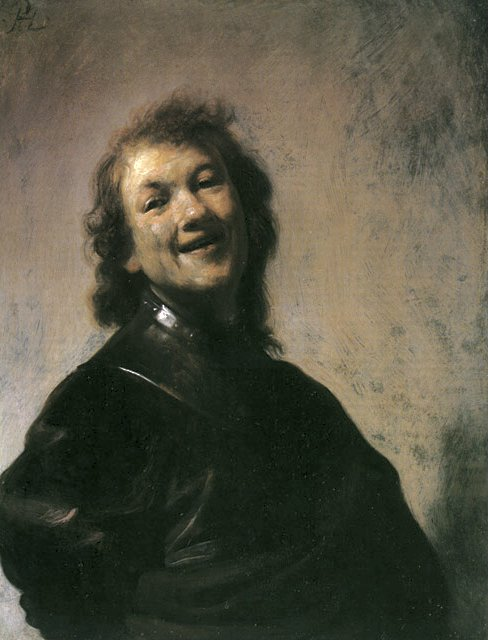
\includegraphics{Rembrandt_self-portrait_1629}
\par\end{centering}

\protect\caption{\label{fig:Rembrandt,-The-Young}Rembrandt, The Young Rembrandt as
Democritus (c. 460 \textendash{} c. 370 BC) the Laughing Philosopher
(1628-1629).}
\end{figure}


Nunc age iam deinceps cunctarum exordia rerum qualia sint et quam
longe distantia formis percipe, multigenis quam sint variata figuris;
non quo multa parum simili sint praedita forma, sed quia non volgo
paria omnibus omnia constant. nec mirum; nam cum sit eorum copia tanta
ut neque finis, uti docui, neque summa sit ulla, debent nimirum non
omnibus omnia prorsum esse pari filo similique adfecta figura.
\begin{eqnarray}
G_{\alpha\beta}\delta g^{\alpha\beta} & = & G_{\alpha\beta}\delta\left(g^{\alpha\nu}g^{\beta\mu}g_{\mu\nu}\right)\label{eq:einstein}\\
 & = & G_{\alpha\beta}g^{\alpha\nu}g^{\beta\mu}\delta g_{\mu\nu}+G_{\alpha\beta}g^{\beta\mu}g_{\mu\nu}\delta g^{\alpha\nu}+G_{\alpha\beta}g^{\alpha\nu}g_{\mu\nu}\delta g^{\beta\mu}\\
 & = & G^{\mu\nu}\delta g_{\mu\nu}+2G_{\alpha\beta}\delta g^{\alpha\beta}\\
 & = & -G^{\mu\nu}\delta g_{\mu\nu}
\end{eqnarray}


Nunc \eqref{eq:einstein} age iam deinceps cunctarum exordia rerum
qualia sint et quam longe distantia formis percipe, multigenis quam
sint variata figuris; non quo multa parum simili sint praedita forma,
sed quia non volgo paria omnibus omnia constant. nec mirum; nam cum
sit eorum copia tanta ut neque finis, uti docui, neque summa sit ulla,
debent nimirum non omnibus omnia prorsum esse pari filo similique
adfecta figura.


\section{Omnibus Omnia Constant}

Nunc age iam deinceps cunctarum exordia rerum qualia sint et quam
longe distantia formis percipe, multigenis quam sint variata figuris;
non quo multa parum simili sint praedita forma, sed quia non volgo
paria omnibus omnia constant. nec mirum; nam cum sit eorum copia tanta
ut neque finis, uti docui, neque summa sit ulla, debent nimirum non
omnibus omnia prorsum esse pari filo similique adfecta figura.Nunc
age iam deinceps cunctarum exordia rerum qualia sint et quam longe
distantia formis percipe, multigenis quam sint variata figuris; non
quo multa parum simili sint praedita forma, sed quia non volgo paria
omnibus omnia constant. nec mirum; nam cum sit eorum copia tanta ut
neque finis, uti docui, neque summa sit ulla, debent nimirum non omnibus
omnia prorsum esse pari filo similique adfecta figura.


\part{Omnibus Omnia Constant}

Nunc age iam deinceps cunctarum exordia rerum qualia sint et quam
longe distantia formis percipe, multigenis quam sint variata figuris;
non quo multa parum simili sint praedita forma, sed quia non volgo
paria omnibus omnia constant. nec mirum; nam cum sit eorum copia tanta
ut neque finis, uti docui, neque summa sit ulla, debent nimirum non
omnibus omnia prorsum esse pari filo similique adfecta figura.


\section{Omnibus Omnia Constant}

Nunc age iam deinceps cunctarum exordia rerum qualia sint et quam
longe distantia formis percipe, multigenis quam sint variata figuris;
non quo multa parum simili sint praedita forma, sed quia non volgo
paria omnibus omnia constant. nec mirum; nam cum sit eorum copia tanta
ut neque finis, uti docui, neque summa sit ulla, debent nimirum non
omnibus omnia prorsum esse pari filo similique adfecta figura.Nunc
age iam deinceps cunctarum exordia rerum qualia sint et quam longe
distantia formis percipe, multigenis quam sint variata figuris; non
quo multa parum simili sint praedita forma, sed quia non volgo paria
omnibus omnia constant. nec mirum; nam cum sit eorum copia tanta ut
neque finis, uti docui, neque summa sit ulla, debent nimirum non omnibus
omnia prorsum esse pari filo similique adfecta figura.Omnibus Omnia
Constant


\section{Omnibus Omnia Constant}

Nunc age iam deinceps cunctarum exordia rerum qualia sint et quam
longe distantia formis percipe, multigenis quam sint variata figuris;
non quo multa parum simili sint praedita forma, sed quia non volgo
paria omnibus omnia constant. nec mirum; nam cum sit eorum copia tanta
ut neque finis, uti docui, neque summa sit ulla, debent nimirum non
omnibus omnia prorsum esse pari filo similique adfecta figura.Nunc
age iam deinceps cunctarum exordia rerum qualia sint et quam longe
distantia formis percipe, multigenis quam sint variata figuris; non
quo multa parum simili sint praedita forma, sed quia non volgo paria
omnibus omnia constant. nec mirum; nam cum sit eorum copia tanta ut
neque finis, uti docui, neque summa sit ulla, debent nimirum non omnibus
omnia prorsum esse pari filo similique adfecta figura.

Nunc age iam deinceps cunctarum exordia rerum qualia sint et quam
longe distantia formis percipe, multigenis quam sint variata figuris;
non quo multa parum simili sint praedita forma, sed quia non volgo
paria omnibus omnia constant. nec mirum; nam cum sit eorum copia tanta
ut neque finis, uti docui, neque summa sit ulla, debent nimirum non
omnibus omnia prorsum esse pari filo similique adfecta figura.Nunc
age iam deinceps cunctarum exordia rerum qualia sint et quam longe
distantia formis percipe, multigenis quam sint variata figuris; non
quo multa parum simili sint praedita forma, sed quia non volgo paria
omnibus omnia constant. nec mirum; nam cum sit eorum copia tanta ut
neque finis, uti docui, neque summa sit ulla, debent nimirum non omnibus
omnia prorsum esse pari filo similique adfecta figura.


\part*{Conclusion}

Nunc age iam deinceps cunctarum exordia rerum qualia sint et quam
longe distantia formis percipe, multigenis quam sint variata figuris;
non quo multa parum simili sint praedita forma, sed quia non volgo
paria omnibus omnia constant. nec mirum; nam cum sit eorum copia tanta
ut neque finis, uti docui, neque summa sit ulla, debent nimirum non
omnibus omnia prorsum esse pari filo similique adfecta figura.

\bibliographystyle{JHEP}
\phantomsection\addcontentsline{toc}{section}{\refname}\bibliography{refs}

\end{document}
